%
% blocks.tex -- slide template
%
% (c) 2021 Prof Dr Andreas Müller, OST Ostschweizer Fachhochschule
%
\bgroup
\def\s{0.4}
\def\punkt#1#2{({#1*\s},{(3-#2)*\s})}
\def\feld#1#2#3{
        \fill[color=#3] \punkt{(#1-0.5)}{(#2+0.5)}
		rectangle \punkt{(#1+0.5)}{(#2-0.5)};
}
\definecolor{darkgreen}{rgb}{0,0.6,0}
\begin{frame}[t]
\setlength{\abovedisplayskip}{5pt}
\setlength{\belowdisplayskip}{5pt}
\frametitle{Blocks}
\vspace{-20pt}
\begin{columns}[t,onlytextwidth]
\begin{column}{0.48\textwidth}
\begin{block}{Blocks}
$4\times k$ Matrizen mit $k=4,\dots,8$
\begin{center}
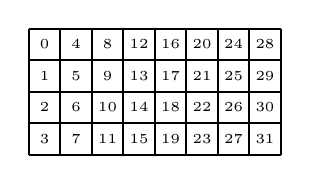
\begin{tikzpicture}[>=latex,thick]
\xdef\s{0.4}
\foreach \i in {0,...,31}{
	\pgfmathparse{mod(\i,4)}
	\xdef\y{\pgfmathresult}
	\pgfmathparse{int(\i/4)}
	\xdef\x{\pgfmathresult}
	\node at \punkt{\x}{\y} {\tiny $\i$};
}
\foreach \x in {-0.5,0.5,...,7.5}{
	\draw \punkt{\x}{-0.5} -- \punkt{\x}{3.5};
}
\foreach \y in {-0.5,0.5,...,3.5}{
	\draw \punkt{-0.5}{\y} -- \punkt{7.5}{\y};
}
\end{tikzpicture}
\end{center}
\uncover<2->{%
Spalten sind $4$-dimensionale $\mathbb{F}_{2^8}$-Vektoren
}
\end{block}
\uncover<3->{%
\begin{block}{Zeilenshift}
\begin{center}
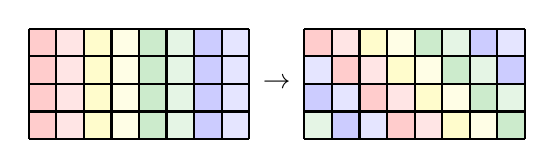
\begin{tikzpicture}[>=latex,thick]

\xdef\s{0.35}

\begin{scope}
	\feld{0}{3}{red!20}
	\feld{0}{2}{red!20}
	\feld{0}{1}{red!20}
	\feld{0}{0}{red!20}

	\feld{1}{3}{red!10}
	\feld{1}{2}{red!10}
	\feld{1}{1}{red!10}
	\feld{1}{0}{red!10}

	\feld{2}{3}{yellow!20}
	\feld{2}{2}{yellow!20}
	\feld{2}{1}{yellow!20}
	\feld{2}{0}{yellow!20}

	\feld{3}{3}{yellow!10}
	\feld{3}{2}{yellow!10}
	\feld{3}{1}{yellow!10}
	\feld{3}{0}{yellow!10}

	\feld{4}{3}{darkgreen!20}
	\feld{4}{2}{darkgreen!20}
	\feld{4}{1}{darkgreen!20}
	\feld{4}{0}{darkgreen!20}

	\feld{5}{3}{darkgreen!10}
	\feld{5}{2}{darkgreen!10}
	\feld{5}{1}{darkgreen!10}
	\feld{5}{0}{darkgreen!10}

	\feld{6}{3}{blue!20}
	\feld{6}{2}{blue!20}
	\feld{6}{1}{blue!20}
	\feld{6}{0}{blue!20}

	\feld{7}{3}{blue!10}
	\feld{7}{2}{blue!10}
	\feld{7}{1}{blue!10}
	\feld{7}{0}{blue!10}

	\foreach \x in {-0.5,0.5,...,7.5}{
		\draw \punkt{\x}{-0.5} -- \punkt{\x}{3.5};
	}
	\foreach \y in {-0.5,0.5,...,3.5}{
		\draw \punkt{-0.5}{\y} -- \punkt{7.5}{\y};
	}
\end{scope}

\begin{scope}[xshift=3.5cm]
        \feld{0}{0}{red!20}
        \feld{1}{1}{red!20}
        \feld{2}{2}{red!20}
        \feld{3}{3}{red!20}

        \feld{1}{0}{red!10}
        \feld{2}{1}{red!10}
        \feld{3}{2}{red!10}
        \feld{4}{3}{red!10}

        \feld{2}{0}{yellow!20}
        \feld{3}{1}{yellow!20}
        \feld{4}{2}{yellow!20} \feld{5}{3}{yellow!20}

        \feld{3}{0}{yellow!10}
        \feld{4}{1}{yellow!10}
        \feld{5}{2}{yellow!10}
        \feld{6}{3}{yellow!10}

        \feld{4}{0}{darkgreen!20}
        \feld{5}{1}{darkgreen!20}
        \feld{6}{2}{darkgreen!20}
        \feld{7}{3}{darkgreen!20}

        \feld{5}{0}{darkgreen!10}
        \feld{6}{1}{darkgreen!10}
        \feld{7}{2}{darkgreen!10}
        \feld{0}{3}{darkgreen!10}

        \feld{6}{0}{blue!20}
        \feld{7}{1}{blue!20}
        \feld{0}{2}{blue!20}
        \feld{1}{3}{blue!20}

        \feld{7}{0}{blue!10}
        \feld{0}{1}{blue!10}
        \feld{1}{2}{blue!10}
        \feld{2}{3}{blue!10}

	\foreach \x in {-0.5,0.5,...,7.5}{
		\draw \punkt{\x}{-0.5} -- \punkt{\x}{3.5};
	}
	\foreach \y in {-0.5,0.5,...,3.5}{
		\draw \punkt{-0.5}{\y} -- \punkt{7.5}{\y};
	}

	\node at \punkt{-1.5}{1.5} {$\rightarrow$};
\end{scope}

\end{tikzpicture}
\end{center}
\end{block}}
\end{column}
\begin{column}{0.50\textwidth}
\uncover<4->{%
\begin{block}{Spalten mischen}
Lineare Operation auf Spaltenvektoren mit Matrix
\begin{align*}
C&=\begin{pmatrix}
\texttt{02}_{16}&\texttt{03}_{16}&\texttt{01}_{16}&\texttt{01}_{16}\\
\texttt{01}_{16}&\texttt{02}_{16}&\texttt{03}_{16}&\texttt{01}_{16}\\
\texttt{01}_{16}&\texttt{01}_{16}&\texttt{02}_{16}&\texttt{03}_{16}\\
\texttt{03}_{16}&\texttt{01}_{16}&\texttt{01}_{16}&\texttt{02}_{16}
\end{pmatrix}
\\
\uncover<5->{
\det C
&=
\texttt{0a}_{16}
}
\uncover<6->{
\ne 0}
\uncover<7->{
\quad\Rightarrow\quad \exists C^{-1}
}
\end{align*}
\end{block}}
\uncover<8->{%
\begin{block}{Als Polynommultiplikation}
Spalten = Polynome in $\mathbb{F}_{2^8}[Z]/(Z^4-1)$,
\\
\uncover<9->{%
$C=\mathstrut$ Multiplikation mit
\[
c(Z) = \texttt{03}_{16}Z^3 + Z^2 + Z + \texttt{02}_{16}
\]
}
\end{block}}
\end{column}
\end{columns}
\end{frame}
\egroup
